\section{SiO2}
\subsection*{Material ID: mp-bfqyx}
\textbf{Constante Dieléctrica ($\epsilon_{total}$):} 4.31 \\[0.5em]
\begin{table}[h!]
\centering
\begin{tabular}{lcc}
\toprule
\textbf{Métrica} & \textbf{Lámina (Plate)} & \textbf{Cilindros (Rod)} \\
\midrule
Bandgaps ($a/\lambda$) & Ninguno & Ninguno \\
Resonancias & 36 & 36 \\
\bottomrule
\end{tabular}
\end{table}
\begin{figure}[H]
\centering
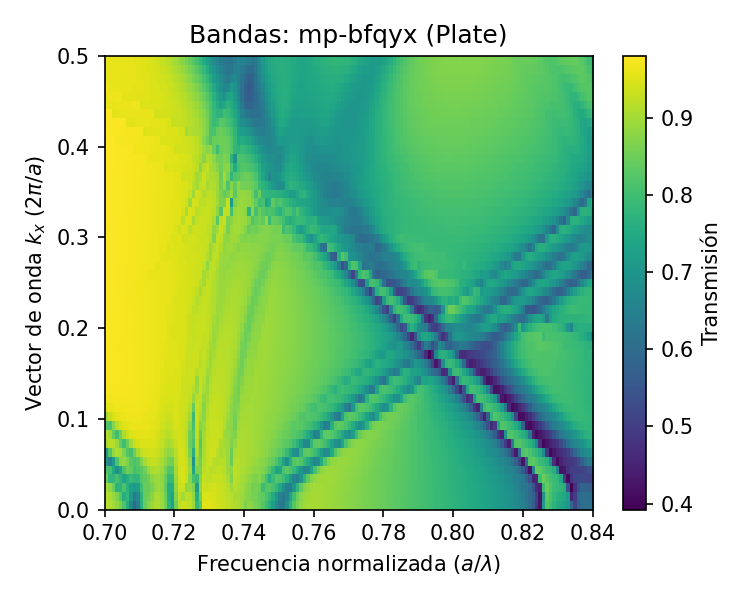
\includegraphics[width=0.48\textwidth]{figures/mp-bfqyx_plate.png}
\hfill
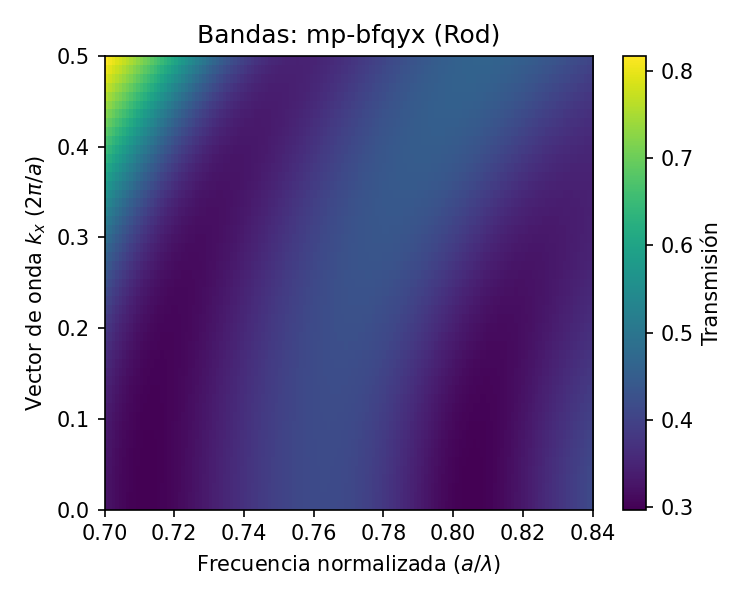
\includegraphics[width=0.48\textwidth]{figures/mp-bfqyx_rod.png}
\caption{Estructuras de bandas fotónicas para mp-bfqyx. Izquierda: Lámina. Derecha: Cilindros.}
\end{figure}
\vspace{1em}
\hrule
\vspace{1em}
\subsection*{Material ID: mp-bfrjg}
\textbf{Constante Dieléctrica ($\epsilon_{total}$):} 6.32 \\[0.5em]
\begin{table}[h!]
\centering
\begin{tabular}{lcc}
\toprule
\textbf{Métrica} & \textbf{Lámina (Plate)} & \textbf{Cilindros (Rod)} \\
\midrule
Bandgaps ($a/\lambda$) & Ninguno & Ninguno \\
Resonancias & 36 & 36 \\
\bottomrule
\end{tabular}
\end{table}
\begin{figure}[H]
\centering
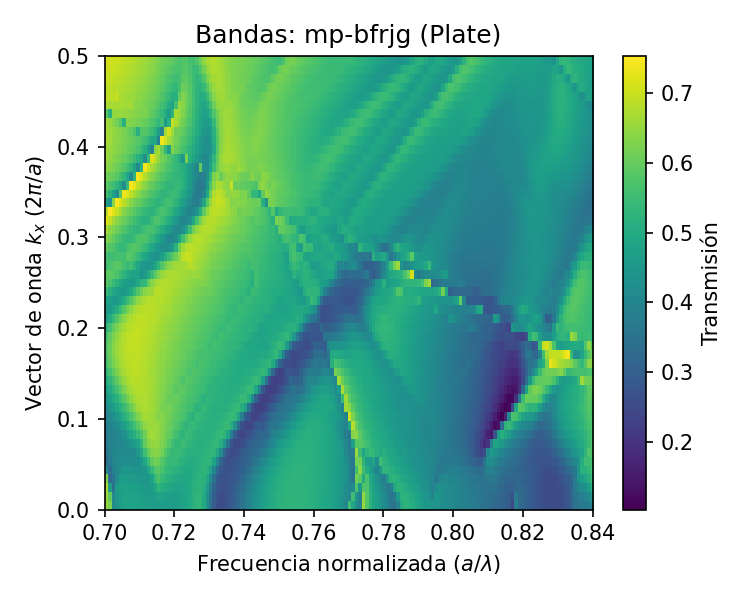
\includegraphics[width=0.48\textwidth]{figures/mp-bfrjg_plate.png}
\hfill
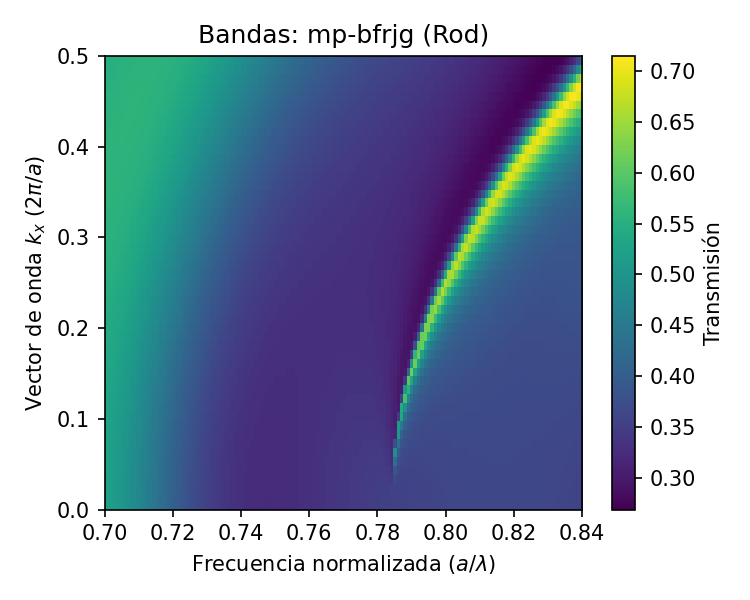
\includegraphics[width=0.48\textwidth]{figures/mp-bfrjg_rod.png}
\caption{Estructuras de bandas fotónicas para mp-bfrjg. Izquierda: Lámina. Derecha: Cilindros.}
\end{figure}
\vspace{1em}
\hrule
\vspace{1em}
\subsection*{Material ID: mp-bfrqy}
\textbf{Constante Dieléctrica ($\epsilon_{total}$):} 4.78 \\[0.5em]
\begin{table}[h!]
\centering
\begin{tabular}{lcc}
\toprule
\textbf{Métrica} & \textbf{Lámina (Plate)} & \textbf{Cilindros (Rod)} \\
\midrule
Bandgaps ($a/\lambda$) & Ninguno & Ninguno \\
Resonancias & 36 & 36 \\
\bottomrule
\end{tabular}
\end{table}
\begin{figure}[H]
\centering
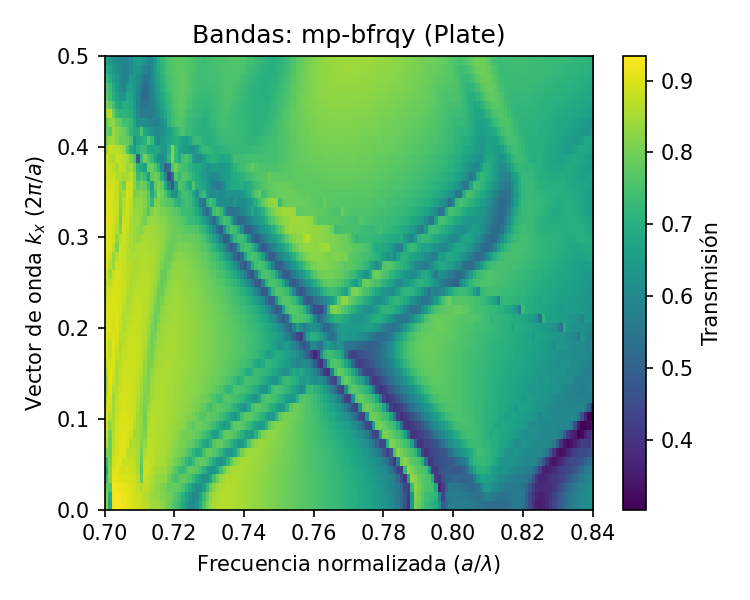
\includegraphics[width=0.48\textwidth]{figures/mp-bfrqy_plate.png}
\hfill
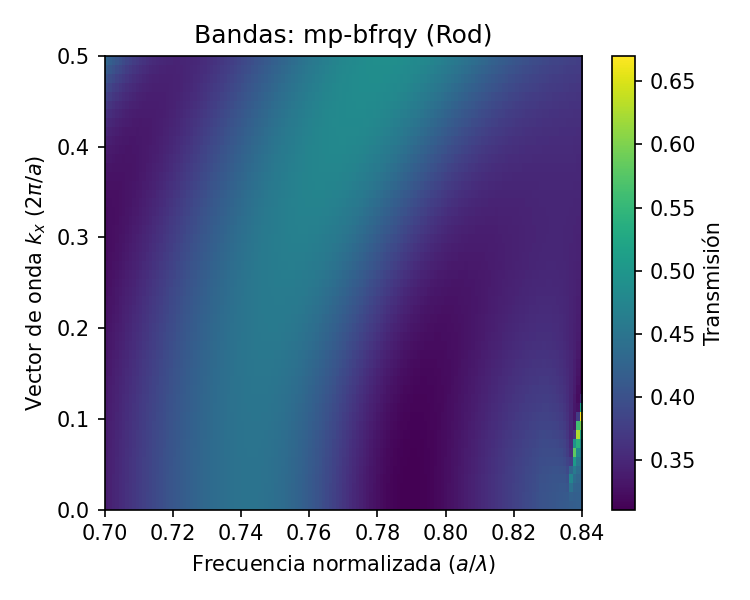
\includegraphics[width=0.48\textwidth]{figures/mp-bfrqy_rod.png}
\caption{Estructuras de bandas fotónicas para mp-bfrqy. Izquierda: Lámina. Derecha: Cilindros.}
\end{figure}
\vspace{1em}
\hrule
\vspace{1em}
\subsection*{Material ID: mp-bfrum}
\textbf{Constante Dieléctrica ($\epsilon_{total}$):} 4.25 \\[0.5em]
\begin{table}[h!]
\centering
\begin{tabular}{lcc}
\toprule
\textbf{Métrica} & \textbf{Lámina (Plate)} & \textbf{Cilindros (Rod)} \\
\midrule
Bandgaps ($a/\lambda$) & Ninguno & Ninguno \\
Resonancias & 36 & 36 \\
\bottomrule
\end{tabular}
\end{table}
\begin{figure}[H]
\centering
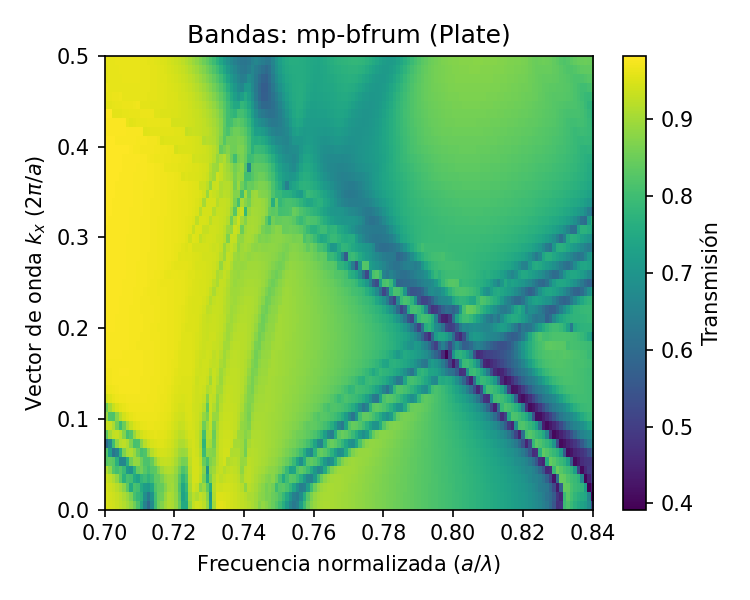
\includegraphics[width=0.48\textwidth]{figures/mp-bfrum_plate.png}
\hfill
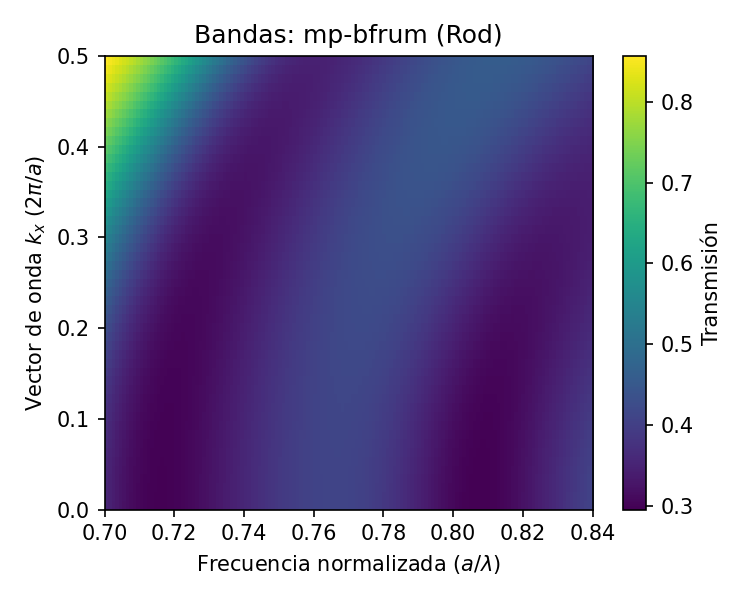
\includegraphics[width=0.48\textwidth]{figures/mp-bfrum_rod.png}
\caption{Estructuras de bandas fotónicas para mp-bfrum. Izquierda: Lámina. Derecha: Cilindros.}
\end{figure}
\vspace{1em}
\hrule
\vspace{1em}
\subsection*{Material ID: mp-bfryn}
\textbf{Constante Dieléctrica ($\epsilon_{total}$):} 3.47 \\[0.5em]
\begin{table}[h!]
\centering
\begin{tabular}{lcc}
\toprule
\textbf{Métrica} & \textbf{Lámina (Plate)} & \textbf{Cilindros (Rod)} \\
\midrule
Bandgaps ($a/\lambda$) & Ninguno & Ninguno \\
Resonancias & 36 & 36 \\
\bottomrule
\end{tabular}
\end{table}
\begin{figure}[H]
\centering
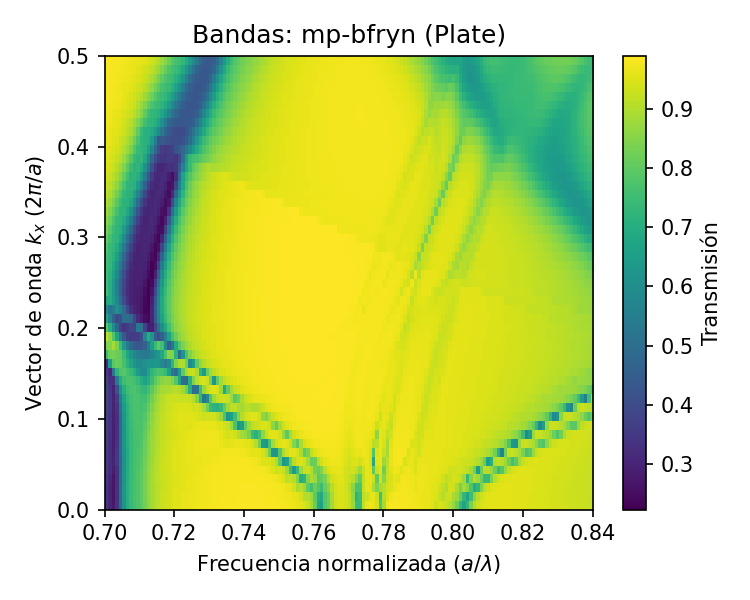
\includegraphics[width=0.48\textwidth]{figures/mp-bfryn_plate.png}
\hfill
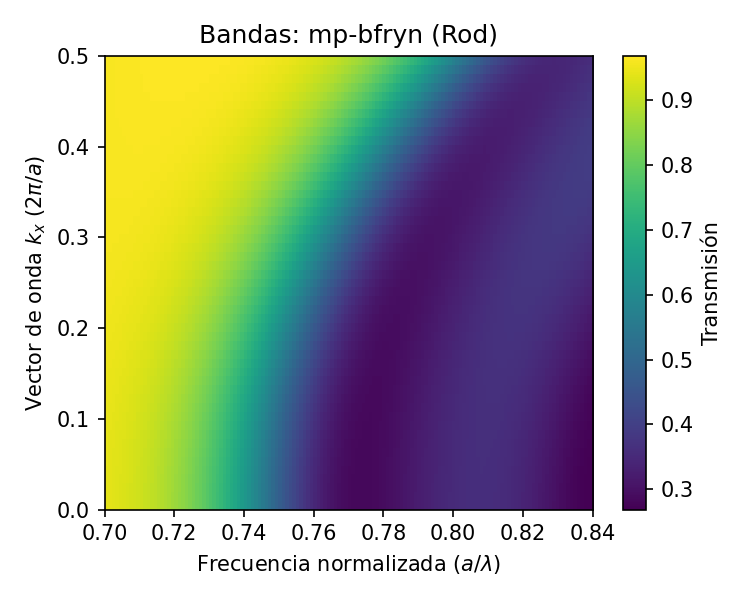
\includegraphics[width=0.48\textwidth]{figures/mp-bfryn_rod.png}
\caption{Estructuras de bandas fotónicas para mp-bfryn. Izquierda: Lámina. Derecha: Cilindros.}
\end{figure}
\vspace{1em}
\hrule
\vspace{1em}
\subsection*{Material ID: mp-bfryw}
\textbf{Constante Dieléctrica ($\epsilon_{total}$):} 3.94 \\[0.5em]
\begin{table}[h!]
\centering
\begin{tabular}{lcc}
\toprule
\textbf{Métrica} & \textbf{Lámina (Plate)} & \textbf{Cilindros (Rod)} \\
\midrule
Bandgaps ($a/\lambda$) & Ninguno & Ninguno \\
Resonancias & 36 & 36 \\
\bottomrule
\end{tabular}
\end{table}
\begin{figure}[H]
\centering
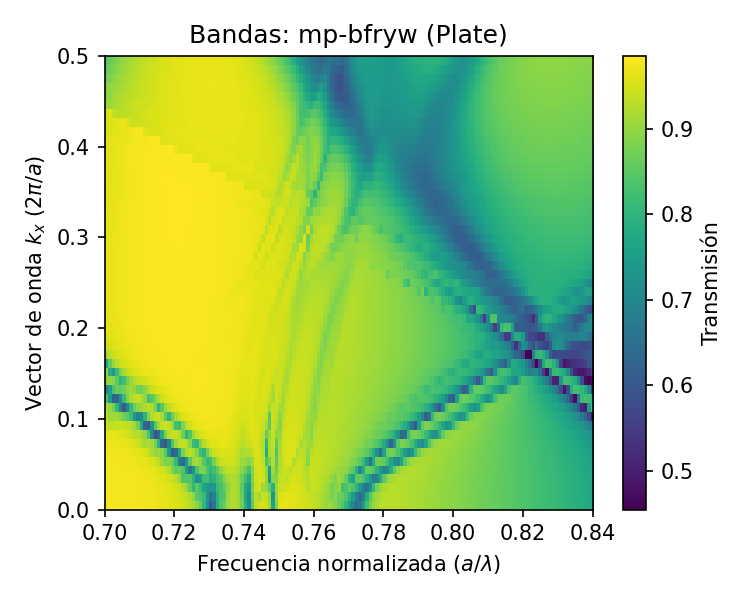
\includegraphics[width=0.48\textwidth]{figures/mp-bfryw_plate.png}
\hfill
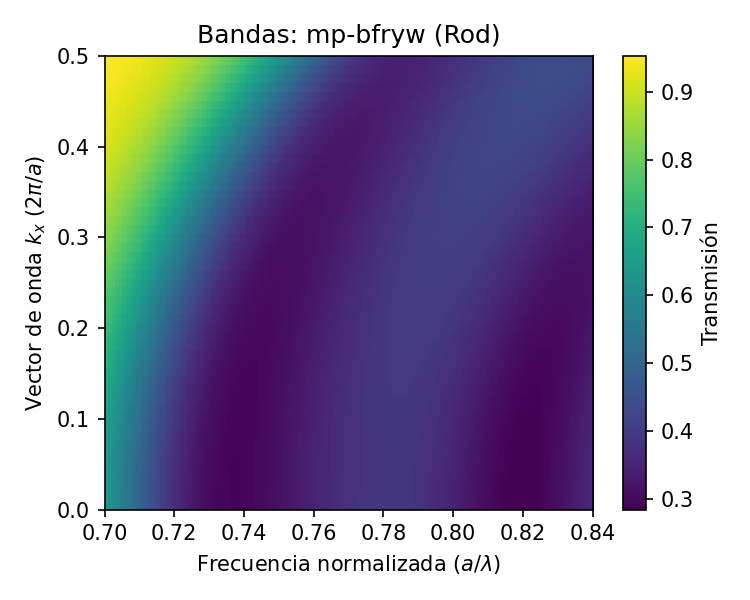
\includegraphics[width=0.48\textwidth]{figures/mp-bfryw_rod.png}
\caption{Estructuras de bandas fotónicas para mp-bfryw. Izquierda: Lámina. Derecha: Cilindros.}
\end{figure}
\vspace{1em}
\hrule
\vspace{1em}
\clearpage